
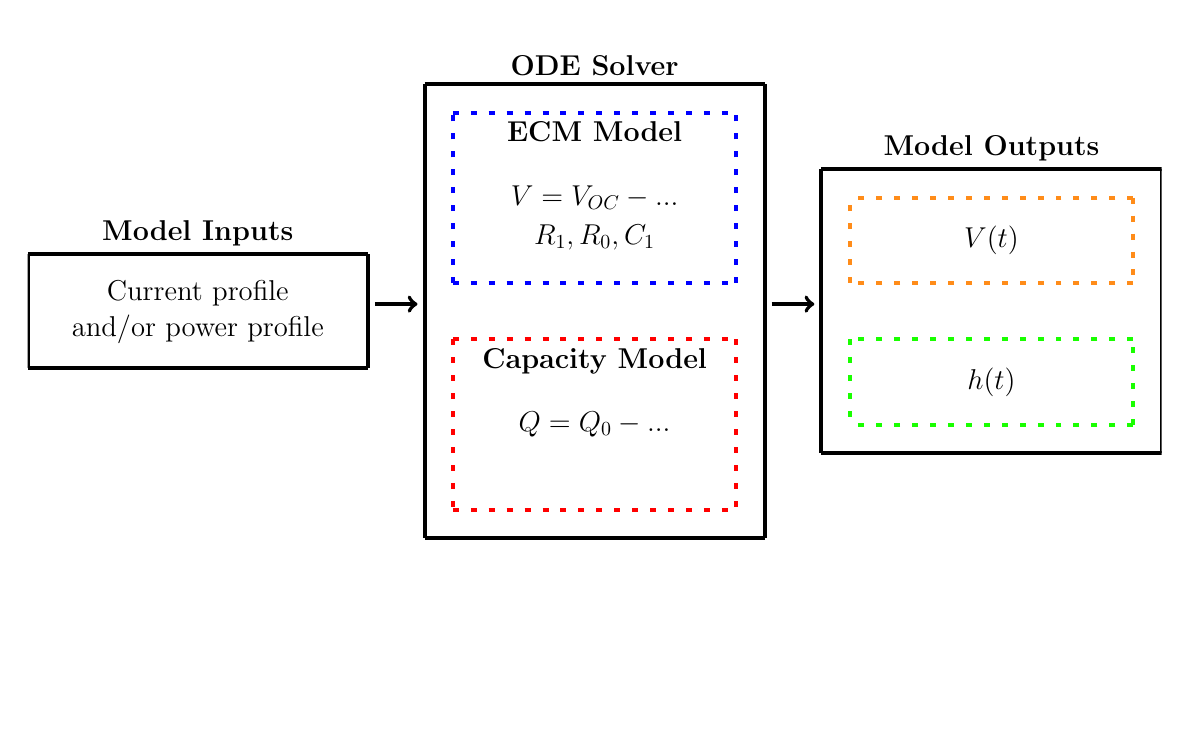
\begin{tikzpicture}[scale=0.72]
  \begin{axis}[
      x=2cm,y=2cm,
      axis lines=middle,
      ymajorgrids=false,
      xmajorgrids=false,
      axis line style={draw=none},
      ticks=none,
      xmin=-3,
      xmax=7,
      ymin=-3,
      ymax=3]
    %\clip(-4,-2) rectangle (4,4);

    \draw (0,0.5) node[anchor=south] (endbox1) {};
    \draw (0.5,0.5) node[anchor=south] (startbox2) {};
    \draw (3.5,0.5) node[anchor=south] (endbox2) {};
    \draw (4,0.5) node[anchor=south] (startbox3) {};

    % input box
    \draw [line width=2pt] (-3,1)-- (-3,0);
    \draw [line width=2pt] (-3,0)-- (0,0);
    \draw [line width=2pt] (0,1)-- (0,0);
    \draw [arrows=->,line width=2pt,draw] (endbox1)--(startbox2);
    \draw [arrows=->,line width=2pt,draw] (endbox2)--(startbox3);

    % ODE box
    \draw[line width = 2pt] (0.5,-1.5) -- (0.5,2.5);
    \draw[line width = 2pt] (0.5,-1.5) -- (3.5,-1.5);
    \draw[line width = 2pt] (3.5,-1.5) -- (3.5,2.5);

    % ECM model
    \draw[line width = 2pt,loosely dashed,color=blue] (0.75,0.75) -- (0.75,2.25);
    \draw[line width = 2pt,loosely dashed,color=blue] (0.75,0.75) -- (3.25,0.75);
    \draw[line width = 2pt,loosely dashed,color=blue] (3.25,0.75) -- (3.25,2.25);

    % Capacity Model
    \draw[line width = 2pt,loosely dashed,color=red] (0.75,0.25) -- (0.75,-1.25);
    \draw[line width = 2pt,loosely dashed,color=red] (3.25,0.25) -- (3.25,-1.25);
    \draw[line width = 2pt,loosely dashed,color=red] (0.75,-1.25) -- (3.25,-1.25);

    % output box
    \draw[line width = 2pt] (4,-0.75) -- (4,1.75);
    \draw[line width = 2pt] (4,-0.75) -- (7,-0.75);
    \draw[line width = 2pt] (7,-0.75) -- (7,1.75);

    % soh box
    \draw[line width = 2pt,loosely dashed,color=green!90!yellow] (4.25,0.25) -- (4.25,-0.5);
    \draw[line width = 2pt,loosely dashed,color=green!90!yellow] (6.75,0.25) -- (4.25,0.25);
    \draw[line width = 2pt,loosely dashed,color=green!90!yellow] (6.75,-0.5) -- (4.25,-0.5);
    \draw[line width = 2pt,loosely dashed,color=green!90!yellow] (6.75,-0.5) -- (6.75,0.25);

    % voltage box
    \draw[line width = 2pt,loosely dashed,color=orange!90] (4.25,0.75) -- (4.25,1.5);
    \draw[line width = 2pt,loosely dashed,color=orange!90] (6.75,0.75) -- (4.25,0.75);
    \draw[line width = 2pt,loosely dashed,color=orange!90] (6.75,1.5) -- (4.25,1.5);
    \draw[line width = 2pt,loosely dashed,color=orange!90] (6.75,1.5) -- (6.75,0.75);

    % box labels
    \draw [line width=2pt] (0,1)-- (-3,1) node [midway, above] (inputs) {\Large \textbf{Model Inputs}};
    \draw[line width = 2pt] (0.5,2.5) -- (3.5,2.5) node [midway,above] (ode) {\Large \textbf{ODE Solver}};
    \draw[line width = 2pt] (4,1.75) -- (7,1.75) node [midway,above] (outputs) {\Large \textbf{Model Outputs}};

    \draw[line width = 2pt,loosely dashed,color=blue] (0.75,2.25) -- (3.25,2.25) node [midway,below] (ecm) {\textcolor{black}{\Large \textbf{ECM Model}}};
    \draw[line width = 2pt,loosely dashed,color=red] (0.75,0.25) -- (3.25,0.25) node [midway,below] (capacity) {\textcolor{black}{\Large \textbf{Capacity Model}}};
    %\draw[line width = 2pt] (4,1.75) -- (7,1.75) node [midway,above] (outputs) {Outputs};

    % box descriptions
    \draw (-1.5,0.5) node (inputs) {\Large \begin{tabular}{c} Current profile \\ and/or power profile \end{tabular}};

    \node at (5.5,1.125) (voltout) {\Large $V(t)$};
    \node at (2,1.50) (ecmtext1) {\Large $V = V_{OC} -...$};
    \node at (2,1.15) (ecmtext2) {\Large $R_1,R_0,C_1$};
    \node at (5.5,-0.125) (sohout) {\Large $h(t)$};

    \node at (2,-0.50) (captext1) {\Large $Q = Q_0 - ...$};
    %\draw[color=black] (-1.5,1.2) node {Input Profiles};
  \end{axis}
\end{tikzpicture}
